\chapter{Methodology}\label{ch:methodology}

The variables for resilience can be represented in the form of a digraph for exhibiting the inter-dependencies between them in terms of nodes and arcs (\citeauthor{soni2014measuring}, \citeyear{soni2014measuring}). These variables are assigned a value and are put in a matrix. The value obtained from the matrix is compared to the predetermined ideal resilience index to obtain the relative resilience index of the supply chain. The limitation of this research is that it only provides a methodology for measuring the existing resilience of a supply chain, but it does not account for improving the resilience of the supply chain. The methodology proposed in our study aims at improving the existing resilience of a supply chain for better performance under the conditions of uncertainties. 

In our study, we have considered the Agent-based simulation as our primary methodology for illustrating our supply chain model and accounting for disruptions. The supply chain model consists of `S' Suppliers, `M' Manufacturers, `D' Distributors, and `R' Retailers. Each facility acts as an individual agent which has been placed across the United States. The model represents the supply chain of one company having different facilities throughout the country. In the event of disruption, if any of the facilities gets shut down, then they have an alternative facility to turn to in order to get their demands satisfied. In the meantime, the facility that has been affected by the disruption is revived by taking the correct measures to increase the resiliency. Each facility has been assigned certain parameters of cost, time and demand fulfillment rate. There is a constant flow of materials downwards through the agents in the supply chain, while there is a constant flow of information upwards through the agents in the supply chain. It is important that this flow is never interrupted for the efficient performance of the system. In order to maintain this flow during disruption, alternate facilities are selected. The alternate facility gets selected based on the best parameter values amongst the available lists of facilities. There are a total of 5 scenarios depicting the source of disruption in the supply chain. The different strategies that need to be taken as per the source of the disruption are encompassed in the model for the purpose of restoration of the disrupted facility. The most efficient and appropriate strategy makes a massive impact on the resiliency of the system.

\section{Vulnerabilities and Capabilities}

There a lot of reasons for the disruptions to occur in the supply chain. Some may arise due to unfavorable natural conditions such as adverse weather, while some may be targeted attacks on firms. The knowledge of the source of disruption is very critical in order to devise proper mitigation strategies. If we know the reason of the disruption, then we can shift our focus on the repairing the most affected factors due to the disruption rather than doing the analysis of all the factors.
 (\citeauthor{Pettit2010}, \citeyear{Pettit2010}) have jotted down these sources and factors as vulnerabilities and capabilities respectively. They have mentioned 6 vulnerabilities that lead to a disruption in the system. A firm should design its supply chain keeping in mind the relation between the vulnerabilities and capabilities. It should not have more capabilities as well as less capabilities. It should have just the perfect number of capabilities. If the company has enforced more capabilities, then there is a loss in capital. Also, if there are less capabilities, then the supply chain is left vulnerable to the disruptions.
 
We have implemented 5 out of the 6 vulnerabilities that act as a source of disruption. These vulnerabilities are as shown in the Fig \ref{Vulnerabilities}. The major problem that occurs during resolving a disruption in a system is the time taken for thorough analysis of the root cause of the problem.


\begin{figure}[H]
  \centering
  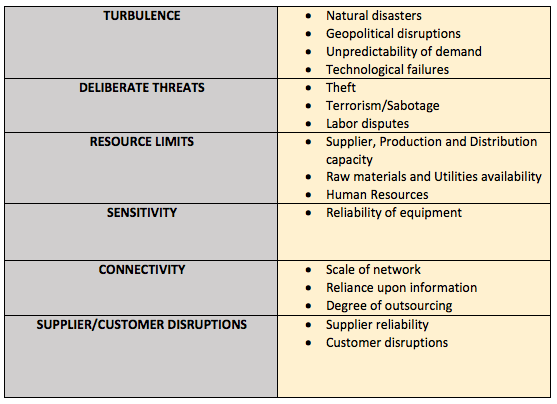
\includegraphics[width=6.5in]{figures/pdf/VNTS.png}\\
  \caption{Vulnerabilities and their various sources.}\label{Vulnerabilities}
\end{figure}


\begin{figure}[H]
  \centering
  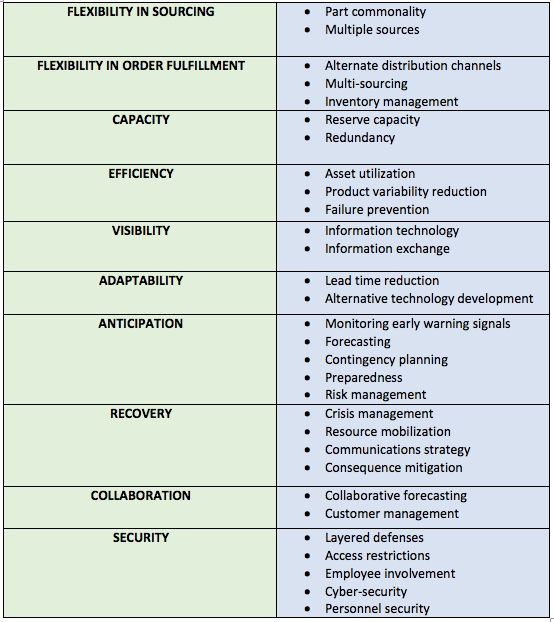
\includegraphics[width=6.0in]{figures/pdf/C1.png}\\
  \caption{Capabilities and their various types.}\label{Capabilities}
\end{figure}

\newpage
 If the managers are well aware of the most common and recurring sources of disruption, they might be able to take preventive and reactive measures during disruptions of similar type in the future. By implementing these vulnerabilities in our supply chain design, we are not only providing ready measures of repair but also reducing the impact of disruption. Thus, making the system both resilient and robust in nature.  
 
Once that the vulnerabilities are addressed, the next step is to glance at the capabilities (factors) that are most likely to be useful for the recovery from the damage from a certain kind of disruption rather looking at all the factors. This will help in reducing the time to find out where the exact problem lies. The list of capabilities that affect the performance of the supply chain system is as shown in Fig \ref{Capabilities}. These capabilities are the measures that help to mitigate the damages that take place because of the disruption.  The vulnerabilities that are closely associated with the capabilities are as shown in the Fig \ref{CV}. These prove to be beneficial in identifying the key factors that can help in improving the speed of recovery of the system back to its functioning state. 



\begin{figure}[H]
  \centering
  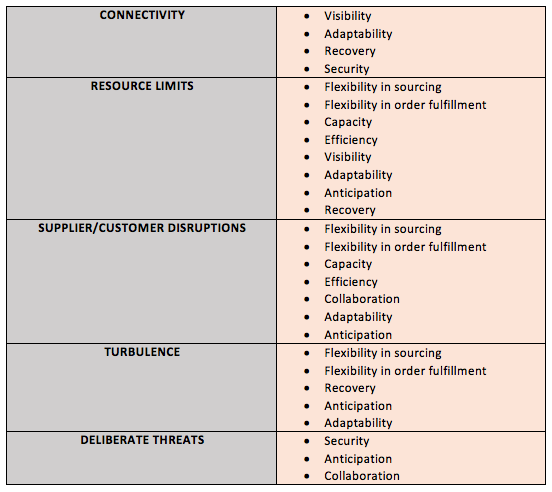
\includegraphics[width=6.0in]{figures/pdf/CV.png}\\
  \caption{Capabilities vs Vulnerabilities.}\label{CV}
\end{figure}




\newpage
\section{Agent-Based Modeling}

The main reason for developing the supply chain model as an agent-based simulation was due to the freedom to express the interaction between agents which is absolutely necessary to consider in our model. The complex nature of the supply chains makes it difficult to design models using the basic simulation models. Agent-based simulation helps in exhibiting the exact nature of a supply chain and all its players. The decision-making, information sharing, uncertainties, trade-offs, and coordination can be accurately represented by the agent-based simulation. It proves as the perfect platform to analyze different strategies and select the best one by implementing in the already existing model. The results are obtained at a fast rate and at an higher accuracy. 

\subsection{The Agents involved}

The model that we have developed for the purpose of our study contains four different agent types and are connected to each other for maintaining a sense of completion. Each agent type has a number of agents that are positioned across the United States of America. If the connections are lost, that means the supply chain has faced a disruption at some point in the network. The description of these agent types and the parameters associated with them are as follows.

\subsubsection{I. Supplier Agent}

These are the facilities that provide the raw materials to the manufacturing facility. The nomenclature for the suppliers has been done as $S_{\text{1}}$, $S_{\text{2}}$, ..., $S_{\text{n}}$. The parameters associated with them are response time (time required to fulfill the demands of the manufacturer) and the raw material handling costs. The costs such as raw material handling cost and inventory holding costs are usually a percentage of the total costs. The percentage value for these costs lies between the range 40 to 60 percent of the total costs (\citeauthor{lee1992managing}, \citeyear{lee1992managing}).
The values corresponding to the response time have ranking from 1 to 3. The rank 1 means that the response time is low, which is highly favorable for the selection criteria. Rank 2 and Rank 3 are the response time medium and high respectively. In the event of disruption, if a supplier is down, then alternate supplier is selected in such a way that the response time is either low or medium, and the raw material handling cost is the minimum.

\subsubsection{II. Manufacturer Agent}

Once the raw material has been acquired from the supplier, it comes to the manufacturer where it is converted into the final product. These manufactures are positioned around the country and their nomenclature is done as $M_{\text{1}}$, $M_{\text{2}}$, ..., $M_{\text{n}}$. The parameters associated with the manufacturer agents are inventory holding cost and response time. In the event of disruption, if any of the manufacturer that fulfills the demands of the distributors associated with it is down, then the alternate manufacturer is selected in such a way that the inventory holding cost is minimum, and the response time is either low or medium. 

\subsubsection{III. Distributor Agent}
The next agent is the distributor agent where the finished goods are collected from the manufacturer and are forwarded to the retailers. The nomenclature for these distributors is done as follows $D_{\text{1}}$, $D_{\text{2}}$, ..., $D_{\text{n}}$. The parameters associated with the distributors are inventory holding cost, order fulfillment rate, and response time. The selection of alternate distributor facility during disruption is done in such a way that the inventory holding cost should be minimum, order fulfillment rate should be high, and the response time should be low or medium. 

\subsubsection{IV. Retailer Agent}
The fourth and final agent in our simulation model is the retailer agent. The retailers accrue the finished products from the distributors depending on the market trends and demands in their respective regions. Some regions have multiple retailers because of the high volume demand of the product from the customers. The nomenclature for the retailers are $R_{\text{1}}$,  $R_{\text{2}}$, ..., $R_{\text{n}}$. A number of different retailer agents are connected to the same distributor agent. The parameter associated with the retailer agent is the response time (to the customers). 



\section{Scenarios in the model}
In a typical supply chain, disruption can occur at any of the levels. Thus, we have developed the scenarios in such a way that the disruptions are occurring at the distributor level, manufacturer level, and the supplier. Also, for all the three events, we have considered the scenarios in which the disruptions are occurring due to the vulnerabilities that have been mentioned earlier. In total, there are 3 different scenarios to quantify the need for our study.

 The flow chart of the our methodology is as show in the Fig \ref{WL}. According to the logic, whenever the disruption occurs, the initial step is to identify the source of the disruption. The next step in the process is to check for the capabilities associated with the source of disruption that is most likely to get affected. During a disruption, it is not necessary that all the capabilities get damaged. Only a certain few capabilities get damaged which hinder with the performance of the system. The final step is to revive those damaged capabilities for getting the system functioning again.
 
The time between the occurrence of disruption and the identification of the key factors is called as the lost time ($T_{\text{L}}$). The time between the identification of the key factors and the total recovery of the disrupted facility is called as the repair time ($T_{\text{N}}$). The time for recovery ($T_{\text{R}}$) is the sum of the lost time ($T_{\text{L}}$) and the time to repair ($T_{\text{N}}$). The total time of the system (T) is the sum of the total cycle time ($T_{\text{C}}$) and the recovery time ($T_{\text{R}}$). 
The ratio of the total time to the recovery time yields the resiliency value ($R_{\text{S}}$)  of the supply chain. 
 
 \begin{equation}
    R_S = \frac{T}{T_R} \label{3.1}
\end{equation}

The higher the value of the resiliency, lesser is the length of recovery of the supply chain during disruption. The percentage change in the resilience value is given by,

\begin{equation}
    \% change in resilience = \frac{R_S(new) - R_S(existing)}{R_S(existing)} * 100
\end{equation}


\begin{figure}[H]
  \centering
  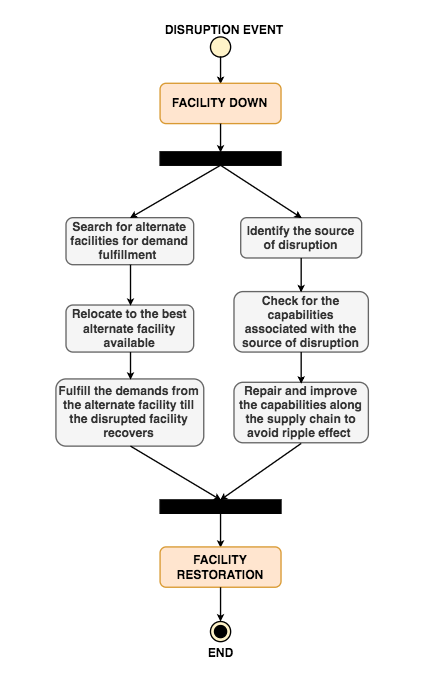
\includegraphics[width=4.0in]{figures/pdf/WL.png}\\
  \caption{Flowchart of Methodology.}\label{WL}
\end{figure}